\documentclass[pract]{SCWorks}
% Тип обучения (одно из значений):
%    bachelor   - бакалавриат (по умолчанию)
%    spec       - специальность
%    master     - магистратура
% Форма обучения (одно из значений):
%    och        - очное (по умолчанию)
%    zaoch      - заочное
% Тип работы (одно из значений):
%    coursework - курсовая работа (по умолчанию)
%    referat    - реферат
%  * otchet     - универсальный отчет
%  * nirjournal - журнал НИР
%  * digital    - итоговая работа для цифровой кафдры
%    diploma    - дипломная работа
%    pract      - отчет о научно-исследовательской работе
%    autoref    - автореферат выпускной работы
%    assignment - задание на выпускную квалификационную работу
%    review     - отзыв руководителя
%    critique   - рецензия на выпускную работу
% Включение шрифта
%    times      - включение шрифта Times New Roman (если установлен)
%                 по умолчанию выключен
\usepackage{preamble}
% \captionsetup[figure]{font= normalsize, labelfont=normalsize}
\renewcommand\theFancyVerbLine{\small\arabic{FancyVerbLine}}

\begin{document}

% Кафедра (в родительном падеже)
\chair{математической кибернетики и компьютерных наук}

% Тема работ
\title{Разработка API web-приложения для организации
процесса уборки мусора}

% Курс
\course{4}

% Группа
\group{451}

% Факультет (в родительном падеже) (по умолчанию "факультета КНиИТ")
% \department{факультета КНиИТ}

% Специальность/направление код - наименование
% \napravlenie{02.03.02 "--- Фундаментальная информатика и информационные технологии}
% \napravlenie{02.03.01 "--- Математическое обеспечение и администрирование информационных систем}
% \napravlenie{09.03.01 "--- Информатика и вычислительная техника}
\napravlenie{09.03.04 "--- Программная инженерия}
% \napravlenie{10.05.01 "--- Компьютерная безопасность}

% Для студентки. Для работы студента следующая команда не нужна.
% \studenttitle{Студентки}

% Фамилия, имя, отчество в родительном падеже
\author{Устюшина Богдана Антоновича}

% Заведующий кафедрой 
\chtitle{доцент, к.\,ф.-м.\,н.}
\chname{С.\,В.\,Миронов}

% Руководитель ДПП ПП для цифровой кафедры (перекрывает заведующего кафедры)
% \chpretitle{
%     заведующий кафедрой математических основ информатики и олимпиадного\\
%     программирования на базе МАОУ <<Ф"=Т лицей №1>>
% }
% \chtitle{г. Саратов, к.\,ф.-м.\,н., доцент}
% \chname{Кондратова\, Ю.\,Н.}

% Научный руководитель (для реферата преподаватель проверяющий работу)
\satitle{профессор, д.\,ф.-м.\,н.} %должность, степень, звание
\saname{В.\,А.\,Романов}

% Руководитель практики от организации (руководитель для цифровой кафедры)
\patitle{профессор, д.\,ф.-м.\,н.}
\paname{В.\,А.\,Романов}

% Руководитель НИР
\nirtitle{профессор, к.\,ф.-м.\,н.} % степень, звание
\nirname{В.\,А.\,Романов}

% Семестр (только для практики, для остальных типов работ не используется)
\term{7}

% Наименование практики (только для практики, для остальных типов работ не
% используется)
\practtype{учебная}

% Продолжительность практики (количество недель) (только для практики, для
% остальных типов работ не используется)
\duration{14}

% Даты начала и окончания практики (только для практики, для остальных типов
% работ не используется)
\practStart{02.09.2024}
\practFinish{08.12.2024}

% Год выполнения отчета
\date{2024}

\maketitle

% Включение нумерации рисунков, формул и таблиц по разделам (по умолчанию -
% нумерация сквозная) (допускается оба вида нумерации)
% \secNumbering

\tableofcontents

% Раздел "Обозначения и сокращения". Может отсутствовать в работе
% \abbreviations
% \begin{description}
%     \item ... "--- ...
%     \item ... "--- ...
% \end{description}

% Раздел "Определения". Может отсутствовать в работе
% \definitions

% Раздел "Определения, обозначения и сокращения". Может отсутствовать в работе.
% Если присутствует, то заменяет собой разделы "Обозначения и сокращения" и
% "Определения"
% \defabbr

\sloppy

\intro

В современном мире проблема загрязнения окружающей среды становится всё более 
актуальной, и мусор, оставляемый на улицах, представляет собой одну из самых 
серьёзных составляющих этой проблемы. Накопление отходов в общественных местах 
не только нарушает эстетический облик городов, но и оказывает негативное 
воздействие на здоровье человека и окружающую экосистему. С каждым годом 
количество бытового и промышленного мусора растёт, и его присутствие на 
улицах городов становится всё более заметным. Это вызывает множество проблем, 
от ухудшения качества воздуха до разрушения экосистем и негативного влияния 
на биоразнообразие.

Мусор, оставляемый на улицах, становится источником различных заболеваний, так 
как разлагающиеся отходы выделяют вредные вещества в воздух и почву. 
Загрязнение воздуха, вызванное гниением мусора, может приводить к серьёзным 
проблемам со здоровьем, таким как аллергические реакции и респираторные 
заболевания. Кроме того, скопление мусора привлекает животных и насекомых, 
что может стать причиной распространения инфекционных заболеваний. Каждый 
элемент уличного мусора, будь то пластиковая бутылка, упаковка или другие 
отходы, способен оказать разрушительное влияние на окружающую среду, нарушая 
естественные экосистемные процессы и угрожая существованию многих видов 
растений и животных.

Ситуация с утилизацией мусора на улицах становится всё более серьёзной. 
Местные власти часто не успевают оперативно реагировать на проблемы, связанные 
с накоплением отходов, из-за нехватки ресурсов и информации о местах их 
скопления. В то же время, население не всегда осведомлено о правильных 
способах утилизации мусора и необходимости поддержания чистоты в своём 
окружении. Поэтому крайне важно не только повышать уровень экологической 
осведомлённости граждан, но и предоставлять им удобные инструменты для 
сообщения о проблемах, связанных с мусором на улицах.

Современные технологии, особенно мобильные приложения, могут стать важным 
инструментом в борьбе с проблемой мусора на улицах. Мобильные платформы 
позволяют быстро и эффективно информировать местные власти о проблемах с 
загрязнением, а также организовывать взаимодействие между гражданами и 
ответственными службами. В рамках своей курсовой работы я разрабатываю 
приложение, которое позволит жителям оперативно сообщать о местах, где 
скопился мусор на улицах, и помогать ответственным службам быстрее устранять 
эти нарушения.

Моё приложение станет платформой для гражданского взаимодействия, где каждый 
пользователь сможет внести свой вклад в улучшение чистоты в своём городе. 
Пользователи смогут легко отправлять сообщения о местах накопления мусора, 
включая фотографии и описание проблемы. Это даст возможность ответственным 
службам более оперативно реагировать на обращения граждан и принимать меры по 
устранению мусора.

Такой подход позволит создать активное сообщество, заинтересованное в 
поддержании чистоты на улицах. Приложение будет не только инструментом для 
сообщения о проблемах, но и средством повышения осведомлённости населения о 
важности заботы о чистоте окружающей среды. Я надеюсь, что благодаря таким 
инициативам мы сможем привлечь внимание к проблеме мусора на улицах и внести 
реальный вклад в её решение, создавая чистую и здоровую среду для будущих 
поколений.

Целью работы является разработка API веб-приложения для эффективной организации
процесса нахождения и уборки мусора на улицах города.

Для достижения цели необходимо решить следующие задачи:
\begin{enumerate}
    \item Рассмотреть используемые технологии, описать преимущества выбранного 
    стека
    \item Описать архитектуру и структуру построенной информационной системы, 
    backend- и database-сервисов
\end{enumerate}

\section{Обзор используемых технологий}

При разработке современных веб-приложений крайне важно выбирать
надёжные и производительные технологии, которые обеспечат 
масштабируемость, гибкость и лёгкость в обслуживании проекта. 
В своём проекте я использую FastAPI, Alembic, PostgreSQL и Docker. У 
каждой из этих технологий есть важные преимущества, которые делают 
их идеальными для создания стабильных и эффективных систем. 
Рассмотрим более подробно, почему стоит выбрать эти инструменты 
для разработки.

\subsection{FastAPI}

FastAPI — это современный и высокопроизводительный веб-фреймворк
для создания API на языке Python. Его основными преимуществами 
являются скорость, лёгкость в использовании и поддержка асинхронного 
программирования.

FastAPI был разработан с акцентом на высокую производительность
и быстрый отклик. Благодаря использованию асинхронных возможностей 
Python (например, ASGI), он позволяет создавать приложения, 
которые могут обрабатывать множество запросов одновременно, 
что особенно важно для высоконагруженных систем. FastAPI по 
скорости сопоставим с такими популярными фреймворками, 
как Node.js и Go.

Ещё одним из достоинств FastAPI является интуитивно понятный
синтаксис и высокая автоматизация процессов. Фреймворк активно 
использует аннотации типов Python, что позволяет разработчикам 
легко описывать API и генерировать документацию в реальном времени. 
При этом FastAPI автоматически проверяет данные на соответствие 
типам, что существенно снижает количество ошибок и делает код более надёжным.

Также FastAPI генерирует документацию API автоматически с
использованием OpenAPI и Swagger, что очень полезно для 
разработки и тестирования приложений. Документация доступна 
в интерактивном виде и позволяет разработчикам и тестировщикам 
мгновенно видеть, как работает API, а также тестировать его 
функциональность.

Поддержка асинхронного программирования в FastAPI позволяет значительно
ускорить обработку запросов и уменьшить задержки в работе приложения. 
Это особенно полезно для задач, связанных с запросами к базе данных 
или внешним сервисам, где приложение может не блокироваться на время 
выполнения операций.

Несмотря на свою молодость, FastAPI активно развивается и поддерживается
сообществом разработчиков. Для него уже существуют многочисленные 
библиотеки и плагины, что позволяет легко расширять функциональность 
приложения \cite{fastapi,uvicorn}.


\subsection{Alembic}

Alembic — это инструмент для управления миграциями базы данных,
который используется совместно с SQLAlchemy, одним из самых 
популярных ORM-фреймворков для Python. Он играет важную роль в 
управлении версионностью схемы базы данных, особенно в проектах, 
где структура данных постоянно изменяется.

Alembic позволяет легко управлять изменениями в базе данных,
обеспечивая поддержку версионного контроля для схем. Это очень 
важно в процессе разработки, когда структура базы данных может 
изменяться, и необходимо сохранять синхронизацию между кодом 
приложения и его данными.

Alembic умеет автоматически создавать миграции на основе изменений 
в моделях SQLAlchemy. Это существенно упрощает процесс разработки
и снижает вероятность ошибок при ручной настройке схемы базы данных. 
Автоматическая генерация миграций ускоряет рабочий процесс и 
делает его более надёжным.

Одним из важных аспектов управления базами данных является возможность
отката изменений. Alembic предоставляет инструменты для того, чтобы 
откатывать миграции, если внесённые изменения привели к ошибкам 
или некорректным результатам. Это делает процесс обновления базы 
данных более безопасным.

Alembic легко интегрируется с SQLAlchemy, что делает его естественным 
выбором при работе с FastAPI. Эта комбинация позволяет разработчикам 
не только легко создавать и управлять моделями данных, но и оперативно 
вносить изменения в структуру базы данных, сохраняя её 
целостность \cite{alembic,sqlalchemy}.

\subsection{PostgreSQL}

PostgreSQL — это мощная объектно-реляционная система управления 
базами данных (СУБД), которая на протяжении многих лет остаётся 
одним из лидеров среди open-source решений для работы с данными. 
В своём проекте я использую PostgreSQL, и на это есть несколько причин:

PostgreSQL славится своей надёжностью и стабильностью.
Она предоставляет высокую степень защиты данных и обеспечивает 
устойчивость к сбоям, что делает её идеальной для критически 
важных приложений, требующих максимальной сохранности информации.

PostgreSQL отлично масштабируется и поддерживает работу с большими
объёмами данных. Это важное преимущество для приложений, 
которые планируются к расширению в будущем, или для тех, кто 
работает с массивами данных в реальном времени.

В отличие от некоторых других реляционных СУБД, PostgreSQL
поддерживает не только стандартные реляционные структуры данных, 
но и работу с JSON, геоданнымиЮ, используя технологию PostGIS 
и другими сложными типамиданных. Это делает её особенно полезной 
для приложений, которые требуют гибкости в работе с 
разнообразными структурами данных.

PostgreSQL полностью соответствует стандартам SQL, что делает 
её совместимой с большим количеством других систем и инструментов. 
Это позволяет использовать её в самых разных проектах и легко 
переносить на неё существующие базы данных.

PostgreSQL обеспечивает полную поддержку транзакций, что гарантирует 
целостность данных и их сохранность в случае сбоев. Это особенно 
важно для приложений, работающих с финансовыми данными или 
другими критически важными ресурсами.

PostgreSQL является бесплатной и открытой СУБД с огромным
сообществом разработчиков и пользователей. Это не только 
экономически выгодно, но и позволяет гибко настраивать систему 
под конкретные нужды проекта \cite{postgresql}.

\subsection{Docker}

Docker — это платформа для автоматизации развёртывания приложений 
в контейнерах. Контейнеризация позволяет упаковать приложение и 
все его зависимости в единый контейнер, что гарантирует его работу 
в любой среде. Docker стал неотъемлемой частью современных процессов 
разработки и развертывания благодаря своим многочисленным преимуществам.

Одним из ключевых преимуществ Docker является возможность создания 
изолированных контейнеров, в которых выполняется приложение. 
Это означает, что разработчик может быть уверен, что приложение 
будет работать одинаково на любой машине, независимо от её операционной 
системы и установленных зависимостей. Изоляция помогает избежать 
проблем, связанных с несовместимостью версий библиотек или конфигураций 
операционной системы.
    
Docker-контейнеры представляют собой лёгкие и переносимые единицы, 
которые можно запускать на любом сервере или облачном провайдере, 
поддерживающем Docker. Это делает приложение независимым от 
инфраструктуры, на которой оно работает, и упрощает перенос с локального 
окружения на серверное. При необходимости легко масштабировать 
приложение, запуская несколько контейнеров на разных узлах.
    
Docker идеально подходит для масштабирования микросервисов и 
распределённых систем. Контейнеры можно легко запускать параллельно, 
что позволяет масштабировать отдельные компоненты приложения в 
зависимости от нагрузки. Это также упрощает поддержку высокой 
доступности и балансировки нагрузки.
    
В отличие от виртуальных машин, которые требуют отдельного ядра 
операционной системы для каждого экземпляра, Docker использует 
ресурсы хоста, что делает контейнеры более лёгкими и менее 
ресурсоёмкими. Это позволяет запускать большее количество контейнеров 
на одном сервере по сравнению с виртуальными машинами.
    
Docker позволяет быстро разворачивать контейнеры, что значительно ускоряет 
процесс деплоя. Контейнеры можно легко обновлять, создавать новые версии 
образов и откатываться к предыдущим версиям при необходимости. Это даёт 
разработчикам и администраторам системы гибкость в управлении версиями 
приложения.
    
Docker позволяет описывать инфраструктуру через Dockerfile, где подробно 
указываются все этапы сборки образа, включая установку зависимостей, 
конфигурацию среды и подготовку приложения к запуску. Это даёт возможность 
легко автоматизировать процесс сборки и развертывания, делая его 
воспроизводимым.
    
Docker имеет огромное сообщество и развивающуюся экосистему. Существует 
множество готовых к использованию контейнеров в Docker Hub, что позволяет 
значительно ускорить процесс разработки за счёт использования существующих 
решений, таких как базы данных, кэш-системы, и другие сервисы.

\subsection{Docker Compose}

В дополнение к Docker я также использую Docker Compose. Docker Compose — это 
инструмент для управления многоконтейнерными приложениями, который изначально
являлся дополнением к контейнерной экосистеме Docker.

Docker Compose позволяет определять и запускать несколько контейнеров Docker 
как единое приложение, что упрощает настройку, управление и масштабирование 
сложных систем. Docker Compose использует файл конфигурации YAML для описания 
всех сервисов, их зависимостей, сетей и томов, необходимых для корректной 
работы приложения.

Docker Compose даёт возможность запускать одновременно несколько контейнеров, 
которые взаимодействуют друг с другом. Например, в рамках одного проекта могут 
быть контейнеры для веб-сервера, базы данных, кеширования и других сервисов. 
Это особенно полезно для микросервисной архитектуры, где каждое приложение 
состоит из множества взаимосвязанных компонентов.
    
Docker Compose использует понятный файл конфигурации 
\texttt{docker-compose.yml}, где описываются все сервисы, их зависимости и 
параметры запуска. Это позволяет легко управлять сложной инфраструктурой и 
делиться конфигурацией с другими разработчиками. Кроме того, этот файл делает 
инфраструктуру воспроизводимой: любой разработчик может развернуть такую же 
среду у себя локально, используя один и тот же конфигурационный файл.
    
Compose значительно упрощает разработку и тестирование многосоставных 
приложений. С его помощью можно настроить различные окружения (например, 
тестовые и продакшн) с минимальными усилиями. Разработчики могут быстро 
развернуть все необходимые компоненты в контейнерах, не настраивая вручную 
каждую службу.
    
Docker Compose упрощает работу с сетями, что важно для взаимодействия между 
контейнерами. Каждый сервис может находиться в отдельной сети или общаться с 
другими сервисами через виртуальные сети Docker. Это позволяет создавать 
изолированные окружения для разных частей приложения и управлять доступом 
между ними. Кроме того, Docker Compose позволяет настраивать постоянные тома 
для хранения данных, что критически важно для баз данных и других сервисов, 
требующих сохранения состояния.
    
Docker Compose позволяет легко масштабировать приложение, увеличивая 
количество реплик определённых контейнеров. Например, если веб-сервер начинает 
испытывать высокую нагрузку, его можно масштабировать до нескольких экземпляров 
без необходимости изменения конфигурации всего проекта. Это делает 
Docker Compose отличным инструментом для управления как разработкой, так и 
продакшн-средами.
    
Docker Compose может быть легко интегрирован в конвейеры непрерывной 
интеграции и доставки (CI/CD), что делает его полезным не только для 
локальной разработки, но и для автоматизированного развертывания приложений. 
С его помощью можно легко тестировать приложение в среде, максимально 
приближённой к продакшн.
    
Одно из важнейших преимуществ Docker Compose — это возможность запускать весь 
проект одной командой: \texttt{docker-compose up}. Все необходимые контейнеры 
будут автоматически развернуты и запущены, что значительно ускоряет и упрощает 
процесс настройки окружения, особенно для новых разработчиков или тестировщиков.
    
Docker Compose предоставляет удобные инструменты для мониторинга состояния 
контейнеров, их логов и работы в целом. Это упрощает отладку приложений и 
позволяет своевременно находить и устранять возможные проблемы \cite{docker}.

\subsection{Postman}

Postman — это популярный инструмент для разработки, тестирования и 
документирования API, который предоставляет разработчикам удобную среду для 
взаимодействия с сервером. В контексте разработки веб-приложений и API на 
основе FastAPI, PostgreSQL и Docker, использование Postman значительно упрощает 
процесс работы с сервером и помогает повысить качество разработки.

Одно из ключевых преимуществ Postman — это его интуитивно понятный интерфейс, 
который позволяет легко отправлять HTTP-запросы (GET, POST, PUT, DELETE) и 
получать ответы от сервера. При создании приложения с серверной частью, 
тестирование API может быть сложным и занимать много времени, если 
использовать стандартные средства, такие как cURL или встроенные в браузеры 
инструменты разработчика. 

Postman позволяет легко работать с различными методами API, не углубляясь в 
сложности написания запросов вручную. Для каждой точки доступа можно задать 
параметры запроса, тело и заголовки, что позволяет полноценно симулировать 
реальное использование API конечными пользователями. Это особенно полезно для 
проверки маршрутов аутентификации, регистрации, создания заявок и других 
функций, реализованных в приложении \cite{postman}.

\subsection{DBeaver}

Также в своей работе я использовал DBeaver — мощный инструмент для работы с 
реляционными и нереляционными базами данных, который предоставляет удобный 
графический интерфейс для взаимодействия с различными системами управления 
базами данных (СУБД).

Одним из значимых преимуществ DBeaver является возможность визуализации 
структуры базы данных. Инструмент позволяет наглядно отображать связи между 
таблицами, показывать диаграммы зависимостей и структуры данных. 
Это помогает лучше понять архитектуру базы данных, увидеть взаимосвязи между 
сущностями и эффективно планировать дальнейшую работу с данными.

DBeaver позволяет строить диаграммы ERD (Entity-Relationship Diagram), что 
помогает документировать структуру базы данных и делать её более понятной. 
DBeaver также поддерживает инструменты для создания резервных копий баз данных 
и выполнения миграций. Это особенно полезно в контексте разработки, когда 
нужно переносить данные или структуру базы данных с одного окружения на 
другое (или в контейнер) \cite{dbeaver}.

\section{Сценарий использования}

Для того чтобы понять, почему была выбрана данная архитектура базы данных, 
обратимся к User-story пользователя, которая покажет основную последовательность
событий, происходящих в процессе пользования приложением.

Основные сценарии использования приложения
\begin{enumerate}
    \item Создание заявки
    \item Модерация
    \item Принятие заявки
    \item Закрытие заявки
\end{enumerate}

Опишем их более подробно.

\subsection{Регистрация пользователя}

Прежде чем воспользоваться функционалом приложения, пользователю необходимо 
пройти регистрацию. Этот процесс включает в себя создание аккаунта с указанием 
имени пользователя, электронной почты и пароля. 

Регистрация необходима для того, чтобы обеспечить пользователям возможность 
создания заявок, а также контроля за своими действиями, участия в уборке 
территорий и прочим взаимодействии с другими участниками процесса.

\subsection{Создание события (заявки)}

После регистрации и входа в приложение пользователь может создать событие, 
которое представляет собой заявку на уборку мусора. Пользователь может 
указать все необходимые данные проблемы: описание, точный адрес 
места, а также географические координаты (при помощи GPS или карты). 

После ввода всех данных пользователь отправляет заявку, которая сохраняется 
в базе данных приложения и становится доступной для модерации. Таким образом, 
каждый пользователь может легко и оперативно заявить о мусоре, который 
скопился на улице, и инициировать его уборку. 

\subsection{Модерация заявки}

Для обеспечения достоверности информации все созданные пользователями заявки 
проходят этап модерации. Модераторы приложения проверяют, соответствует ли 
указанная информация действительности, и корректно ли описано место 
загрязнения. Это позволяет избежать возможных ошибок или дублирования заявок. 
После проверки заявка либо подтверждается и становится видимой для 
всех пользователей приложения, либо отклоняется, если выявлены несоответствия.

\subsection{Просмотр и выбор заявки пользователями}

После подтверждения заявки модератором, она появляется в общем списке активных 
заявок на уборку. Пользователи приложения могут просматривать эти заявки 
как в виде списка, так и на карте, где все места загрязнений будут отмечены 
специальными метками. В этом интерфейсе каждый пользователь может выбрать ту 
заявку, которая ему удобна по расположению или времени проведения уборки. 
После выбора заявки пользователь может принять её для выполнения. Это 
означает, что он берёт на себя ответственность за уборку данного участка, 
и статус заявки меняется на «Принята». Таким образом, другие пользователи 
видят, что заявка уже находится в процессе выполнения, и могут либо 
присоединиться, либо выбрать другую заявку.

\subsection{Выполнение уборки и закрытие заявки}

Когда пользователь принимает заявку на выполнение, он отправляется на место 
для проведения уборки. После завершения уборки он загружает в приложение 
фотографии, подтверждающие выполнение работы, и отправляет их на проверку 
модератору. Эти фотографии являются доказательством того, что мусор был 
убран, и заявка может быть закрыта. После загрузки фотографий пользователь 
нажимает кнопку «Заявка выполнена», и статус заявки изменяется на «Завершена».
Модератор проверяет предоставленные материалы, и если всё в порядке, заявка 
окончательно закрывается и исчезает из списка активных задач.

\section{Архитектура приложения}

Архитектура приложения, построенного с использованием FastAPI 
и SQLAlchemy, представляет собой современный и популярный 
подход к созданию веб-приложений на Python. Это приложение 
может быть ориентировано на создание и управление RESTful 
API, что делает его подходящим для широкого спектра задач, 
от небольших сервисов до масштабных систем.

Данное приложение использует FastAPI в качестве веб-фреймворка, 
а SQLAlchemy в связке с Alembic — для управления базой данных 
и миграциями. FastAPI является относительно новым веб-фреймворком, 
отличающимся своей скоростью и удобством работы благодаря 
полной поддержке асинхронности и валидации данных на уровне 
запросов с помощью Pydantic. В то же время SQLAlchemy — это 
ORM (Object-Relational Mapping) система, позволяющая работать с базой 
данных на уровне Python-объектов \cite{restapi}.

\subsection{Архитектуры базы данных}

\begin{figure}[H]
	\center{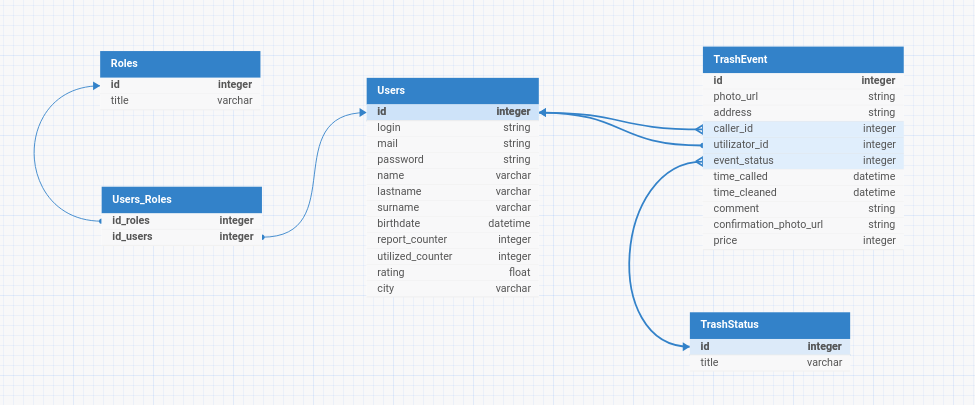
\includegraphics[scale=0.65]{./src/database.png}}
	\caption{Структура проекта}
	\label{pic1}
\end{figure}

На данном скриншоте представлена ER-диаграмма создаваемого сервиса. Основные
сущности приложения, как видно, это Users (пользователи) и TrashEvent (сбор 
мусора). 

Также с помощью отношения many-to-many была реализована ролевая система, 
которая позволяет администратору модерировать создаваемые пользователями заявки.

В таблице TrashStatus, как и было сказано выше, будет описано 4 стадии события.

\subsection{Архитектура backend-сервиса}

Рассмотрим структуру проекта.

\begin{figure}[H]
	\center{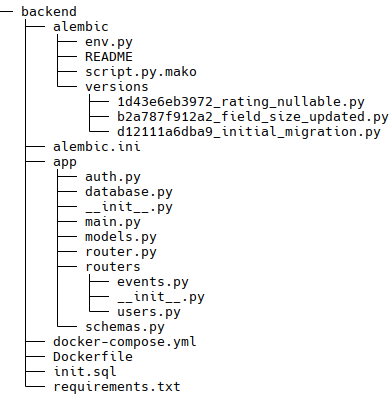
\includegraphics[scale=1.3]{./src/structure.png}}
	\caption{Структура проекта}
	\label{pic2}
\end{figure}

На данном скриншоте представлена основная структура проекта.

Далее опишем файлы в подробности, останавливаясь на самых важных деталях 
реализации.

\subsubsection{Аутентификация}

В файле \texttt{auth.py} реализованы функции для управления аутентификацией 
пользователей. Он использует библиотеку Passlib для хеширования паролей и 
Jose для работы с JSON Web Tokens (JWT) \cite{jwt,oauth2}. Основные функции включают:

\begin{enumerate}
    \item Хеширование пароля (\texttt{get\_password\_hash}) для 
    безопасного хранения паролей в базе данных.
    \item Проверка пароля (\texttt{verify\_password}) для аутентификации 
    пользователей.
    \item Создание токена доступа (\texttt{create\_access\_token}), который 
    выдается после успешной аутентификации и используется для последующих 
    запросов.
\end{enumerate}
    
\subsubsection{База данных}

Файл \texttt{database.py} отвечает за конфигурацию подключения к базе данных 
PostgreSQL. Здесь используется SQLAlchemy для создания движка базы данных, сессий и 
базового класса моделей:
\begin{enumerate}
    \item Создание движка (\texttt{create\_engine}) для работы с PostgreSQL.
    \item Сессии (\texttt{sessionmaker}) для управления транзакциями.
    \item Функция \texttt{get\_db}, которая создает и закрывает сессии базы 
    данных, что позволяет удобно управлять соединениями.
\end{enumerate}

\subsubsection{Основной файл приложения}

В файле \texttt{main.py} создается экземпляр приложения FastAPI и включаются 
маршруты, 
определенные в других модулях. Здесь также вызывается метод для создания всех 
таблиц в базе данных на основе моделей. Это обеспечивает готовность базы 
данных к работе сразу после запуска приложения.

\subsubsection{Модели данных}

Файл \texttt{models.py} определяет модели SQLAlchemy для пользователей и заявок:
\begin{enumerate}
    \item Модель \textbf{User} описывает пользователей с полями, такими как 
    username, email и hashed\_password. Также установлены связи с 
    моделью Request, что позволяет отслеживать заявки, созданные пользователем.
    \item Модель \textbf{TrashEvent} включает такие поля, как description, 
    address, latitude, longitude, status и временные метки. Она также имеет 
    связи с пользователями, которые создали и приняли заявки.
\end{enumerate}
    
\subsubsection{Схемы данных}

В файле \texttt{schemas.py} определены Pydantic схемы, которые используются для 
валидации входящих и исходящих данных. Это позволяет обеспечить целостность 
данных и простоту работы с ними.

Схемы \textbf{UserCreate}, \textbf{UserOut}, \textbf{TrashEventCreate}, и 
\textbf{TrashEventOut} описывают структуру данных, которые приложение ожидает 
получать и отправлять. Это упрощает работу с данными в API и гарантирует, 
что они соответствуют заданной структуре.

\subsubsection{Маршруты}

Файлы маршрутов управляют API-запросами и определяют доступные эндпоинты:
\begin{enumerate}
    \item В \texttt{router.py} реализована аутентификация пользователей с 
    маршрутом для регистрации и логина. Все данные аутентификации 
    обрабатываются через зависимости FastAPI, что упрощает управление токенами.
    \item В \texttt{events.py} находятся маршруты для создания, получения и 
    управления заявками. Это включает:
    \begin{itemize}
        \item Создание новых заявок.
        \item Получение доступных заявок, заявок текущего пользователя и 
        принятых заявок.
        \item Обновление статуса заявок (прием и завершение).
    \end{itemize}
    \item В \texttt{users.py} находятся маршруты для создания, получения и 
    управления заявками. Это включает:
    \begin{itemize}
        \item Получение всех пользователей и текущего пользователя
        \item Изменение данных для пользователя
        \item Удаление пользователя
    \end{itemize}
        
\end{enumerate}
    
\subsubsection{Миграции с использованием Alembic}

Файл \texttt{env.py} является конфигурацией для Alembic, инструмента миграции 
баз данных для SQLAlchemy. Он обеспечивает:
\begin{enumerate}
    \item Подключение к базе данных и управление миграциями.
    \item Автоматическую генерацию миграций на основе изменений в моделях, что 
    позволяет управлять схемой базы данных без потери данных.
\end{enumerate}

В остальном же, в директории \texttt{alembic} находятся файлы, отвечающий за
правильную работу СУБД и работу с миграциями.
    
\subsection{Контейнеризация с помощью Docker и Docker compose}

Опишем более детально процесс контейнеризации, который создан для деплоя 
приложения на любом устройстве.

\subsubsection{Использование базового образа}

\begin{minted}[linenos, breaklines=true, style=bw]{dockerfile}
    FROM python:3.11-slim
\end{minted}

Это минималистичный образ Python, который позволяет создать легковесное 
приложение с низким использованием ресурсов.

\subsubsection{Перенос файлов и зависимостей}

\begin{minted}[linenos, breaklines=true, style=bw]{dockerfile}
    WORKDIR /app
    COPY requirements.txt .
    RUN pip install --no-cache-dir -r requirements.txt
    COPY . .
\end{minted}

Здесь мы устанавливаем рабочую директорию и копируем файл requirements.txt, 
который содержит все необходимые зависимости, в контейнер. Использование флага 
--no-cache-dir помогает уменьшить размер образа, исключая кешированные файлы.

Затем в образ копируется рабочий код, что делает все файлы доступными для 
выполнения.

\subsubsection{Инициализация базы данных}

\begin{minted}[linenos, breaklines=true, style=bw]{dockerfile}
    COPY init.sql /docker-entrypoint-initdb.d/
\end{minted}

Здесь мы копируем SQL-скрипт, который будет автоматически выполнен при 
инициализации базы данных PostgreSQL в контейнере. Этот скрипт создает 
пользователя и базу данных, если они еще не существуют.

\subsubsection{Открытие порта и запуск приложения}

\begin{minted}[linenos, breaklines=true, style=bw]{dockerfile}
    EXPOSE 8000
    CMD ["uvicorn", "app.main:app", "--host", "0.0.0.0", "--port", "8000"]
\end{minted}

Команда \texttt{EXPOSE} указывает, что приложение будет доступно на порту 
8000 внутри, сети Docker, а CMD запускает сервер Uvicorn, который обрабатывает 
входящие запросы.

\subsubsection{Docker Compose}

В \texttt{docker-compose.yml} файле указаны три сервиса, которые отвечают за
работу всего приложения. Это:
\begin{enumerate}
    \item \texttt{web}, образ которого собирается из Dockerfile, описанного 
    выше, а затем монтирует папку для поддержки hot-reload
    \item \texttt{db}, который не дополняется build-файлом и который создаёт
    volume для сохранения данных на локальную машину
    \item \texttt{alembic} — необязательный сервис, который автоматически
    запускает миграции в запущенных контейнерах
\end{enumerate}

\conclusion

Современные технологии, такие как FastAPI, Alembic, PostgreSQL, Docker, Docker 
Compose, Postman и DBeaver, демонстрируют высокую эффективность и 
востребованность в разработке программных решений.

FastAPI — мощный инструмент для создания REST API, отличающийся высокой 
производительностью, удобным синтаксисом и встроенной поддержкой валидации 
данных. Эти характеристики делают его надёжным выбором для реализации 
API-ориентированных проектов.

Alembic обеспечивает удобное управление миграциями базы данных, позволяя 
структурировать изменения схемы и поддерживать согласованность данных. 
Это особенно важно для сложных систем с постоянным развитием.

PostgreSQL выделяется надёжностью, производительностью и гибкостью. Её 
функционал подходит как для сложной аналитики, так и для управления данными 
в высоконагруженных системах.

Docker и Docker Compose предоставляют инструменты для эффективной 
контейнеризации и управления инфраструктурой. Эти технологии обеспечивают 
воспроизводимость окружения и упрощают процесс масштабирования систем.

Postman — удобный инструмент для тестирования API, который помогает 
проверять взаимодействие клиентской и серверной частей, ускоряя процесс 
отладки и повышения качества программного обеспечения.

DBeaver предлагает удобный интерфейс для работы с базой данных, упрощая 
выполнение запросов, анализ данных и работу с SQL-скриптами. Это позволяет 
сосредоточиться на решении задач, связанных с бизнес-логикой.

Использование таких технологий отражает современные тенденции в разработке 
программного обеспечения, позволяя создавать масштабируемые, надёжные и 
высокопроизводительные решения. Их применение способствует повышению качества 
продуктов и облегчает реализацию сложных проектов.

Разработанное приложение представляет собой важный шаг в борьбе 
с загрязнением городской среды, объединяя усилия жителей для решения этой 
актуальной проблемы.

Приложение имеет потенциал для увеличения осведомлённости населения о 
проблемах экологии и вовлечения граждан в активные действия по улучшению 
своей окружающей среды.

\nocite{*}

\inputencoding{cp1251}
\bibliographystyle{gost780uv}
\bibliography{thesis.bib}
\inputencoding{utf8}

\end{document}
